\documentclass{standalone}
\usepackage{pgfplots}

\begin{document}

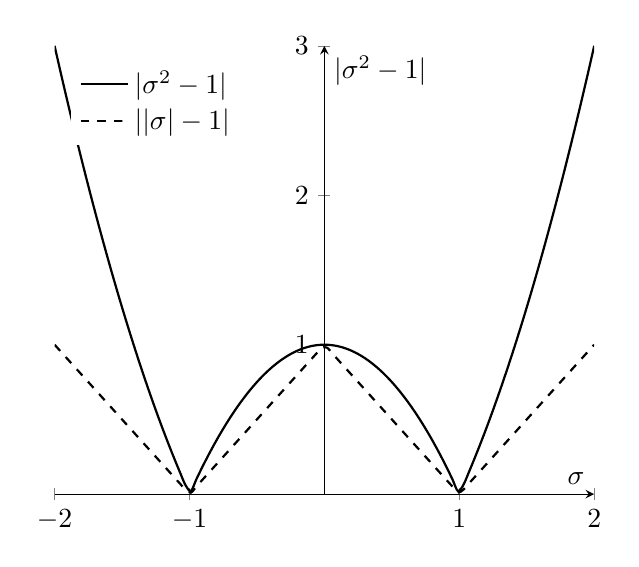
\begin{tikzpicture}
    \begin{axis}[
        axis lines=middle,
        xlabel=$\sigma$,
        ylabel=$| \sigma^2 - 1 |$,
        xmin=-2, xmax=2,
        ymin=0, ymax=3,
        legend pos=north west,
        legend cell align=left,
        legend style={draw=none},
        domain=-2:2,
        samples=100,
        smooth,
        no markers,
        every axis plot/.append style={
            thick,
            mark options={mark size=0pt}
        }
    ]
        \addplot [black, solid] {abs(x^2 - 1)};
        \addlegendentry{$|\sigma^2 - 1|$}
        
        \addplot [black, dashed] {abs(abs(x) - 1)};
        \addlegendentry{$||\sigma|-1|$}
    \end{axis}
\end{tikzpicture}

\end{document}